\chapter{Preparation}
  This chapter details the work done before the main implementation of the project was started. It
  details the devices chosen to implement this project and the reasons for choosing them. It then
  discusses the existing libaries and APIs available for those devices and for the required data
  processing. Finally, it describes software engineering techniques used.

  \section{Requirements analysis}
    The aim of the project is to classify activities based on accelerometer recordings from a consumer smartwatch and smartphone, and evaluate to what extent the smartwatch is better at helping to classify activities. The requirements to accomplish this can be split into two categories: data collection and data processing requirements.
    
    \subsubsection{Data collection requirements}
      \begin{enumerate}
        \item access tri-axial readings from accelerometer on both the smartwatch and the smartphone;
        \item store this accelerometer data temporarily on the internal memory of each device using suitable data structures;
        \item transmit this data from the smartwatch to the smartphone using a suitable protocol;
        \item store the data permanently on the smartphone, to enable transfer to the computer.
      \end{enumerate}
    
    \subsubsection{Data processing requirements}
      \begin{enumerate}
        \item parse the data into a manipulatable format;
        \item preprocess the data, including filtering and splitting into fixed-length bins;
        \item extract features from each bin;
        \item train classifier(s) on the extracted features;
        \item test classifier and record evaluation statistics.
      \end{enumerate}
    
    The remainder of this chapter describes work done to ensure these requirements could be fulfilled.
  
  \section{Introduction to signal processing}
    \label{sec:intro-sig-processing}
    The output from any accelerometer is a time-series representing its acceleration. Effectively extracting information from this time-series is central to the success of this project. Knowledge of signal processing is therefore critical.
    
    It is essential to capture as much of the movement as possible. Conversion from continuous 
    physical acceleration to a discrete time-series requires sampling. The Nyquist-Shannon sampling theorem states that a signal can be exactly reconstructed from its samples if the sample rate is greater than twice the highest frequency of the signal.
    
    The highest frequency of a physical activity is not well defined. The activities I hope to classify will vary in their periodicity. Some, like walking, will be very periodic, while others will have no period at all. Considering common period activities like cycling and walking, I anticipate that the frequencies that best describe movement will be present in the 0--5\si{Hz} range, and so will require sampling at a frequency of at least 10\si{Hz}.
    
    Graphs of accelerometer readings for each of the activities I attempt to classify are presented in section~\ref{sec:activity-details}. 
    
    \subsubsection{Frequency domain analysis}
      Much of the analysis of the accelerometer readings will be done in the frequency domain. A time domain signal can be converted into the frequency domain using a Fourier transform.
      
      The discrete Fourier transform of a sequence of N complex numbers $f_0, f_1, \ldots, f_{N-1}$ is the sequence $F_k$, defined by:
      
      $$F_k = \sum\limits_{n=0}^{N-1} f_n \cdot \mathrm{e}^{-2\pi \mathrm{i} kn/N}$$
      
      The power spectral density, $PSD_k$, of a signal describes how power is distributed over different frequencies. One method of estimating the power spectral density is to take the square of the absolute value of the Fourier transform component:
      
      $$PSD_k = \|F_k\|^2$$
      
    \subsubsection{Noise and filtering}
      The readings from the accelerometer are subject to noise, exhibited in 
      figure~\ref{fig:x_y_z_flat_plot}, which plots readings from the x, y, and z axes during an hour long recording with the chosen smartphone laying flat on a table.
      
      \begin{figure}
        \centering
        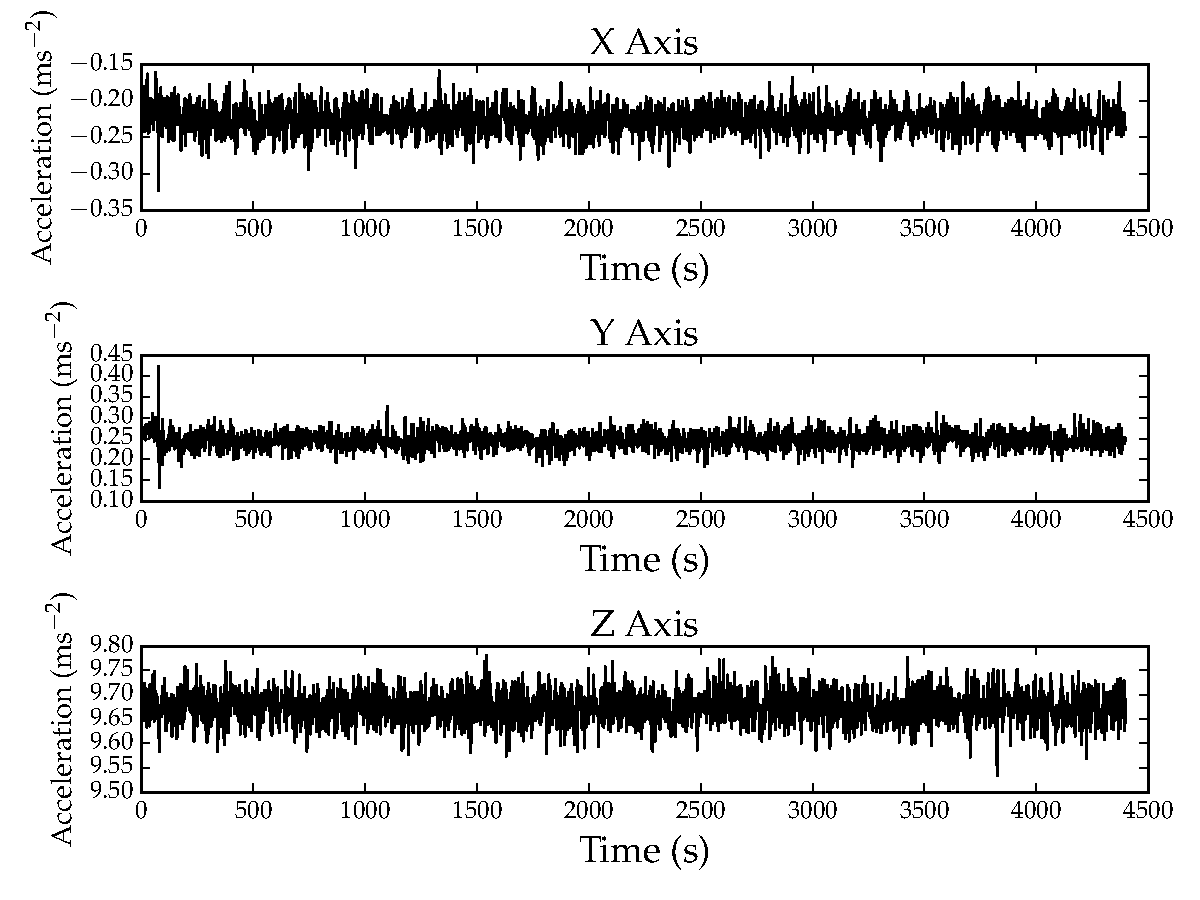
\includegraphics[width=0.8\textwidth]{x_y_z_flat_plot}
        \caption{The x, y and z axis readings from an hour long accelerometer recording of the chosen smartphone laying flat on a table. The readings contain noise.}
        \label{fig:x_y_z_flat_plot}
      \end{figure}
      
      
      Figure~\ref{fig:noise_histogram} plots the distribution of the magnitude of the acceleration, where the magnitude $\|\mathbf{x}\| = \sqrt{x^2+y^2+z^2}$. The magnitude, which should be a constant $\mathrm{g} \approx 9.81 \si{\meter\per\square\second}$, is subject to normally distributed noise.
      
      \begin{figure}
        \centering
        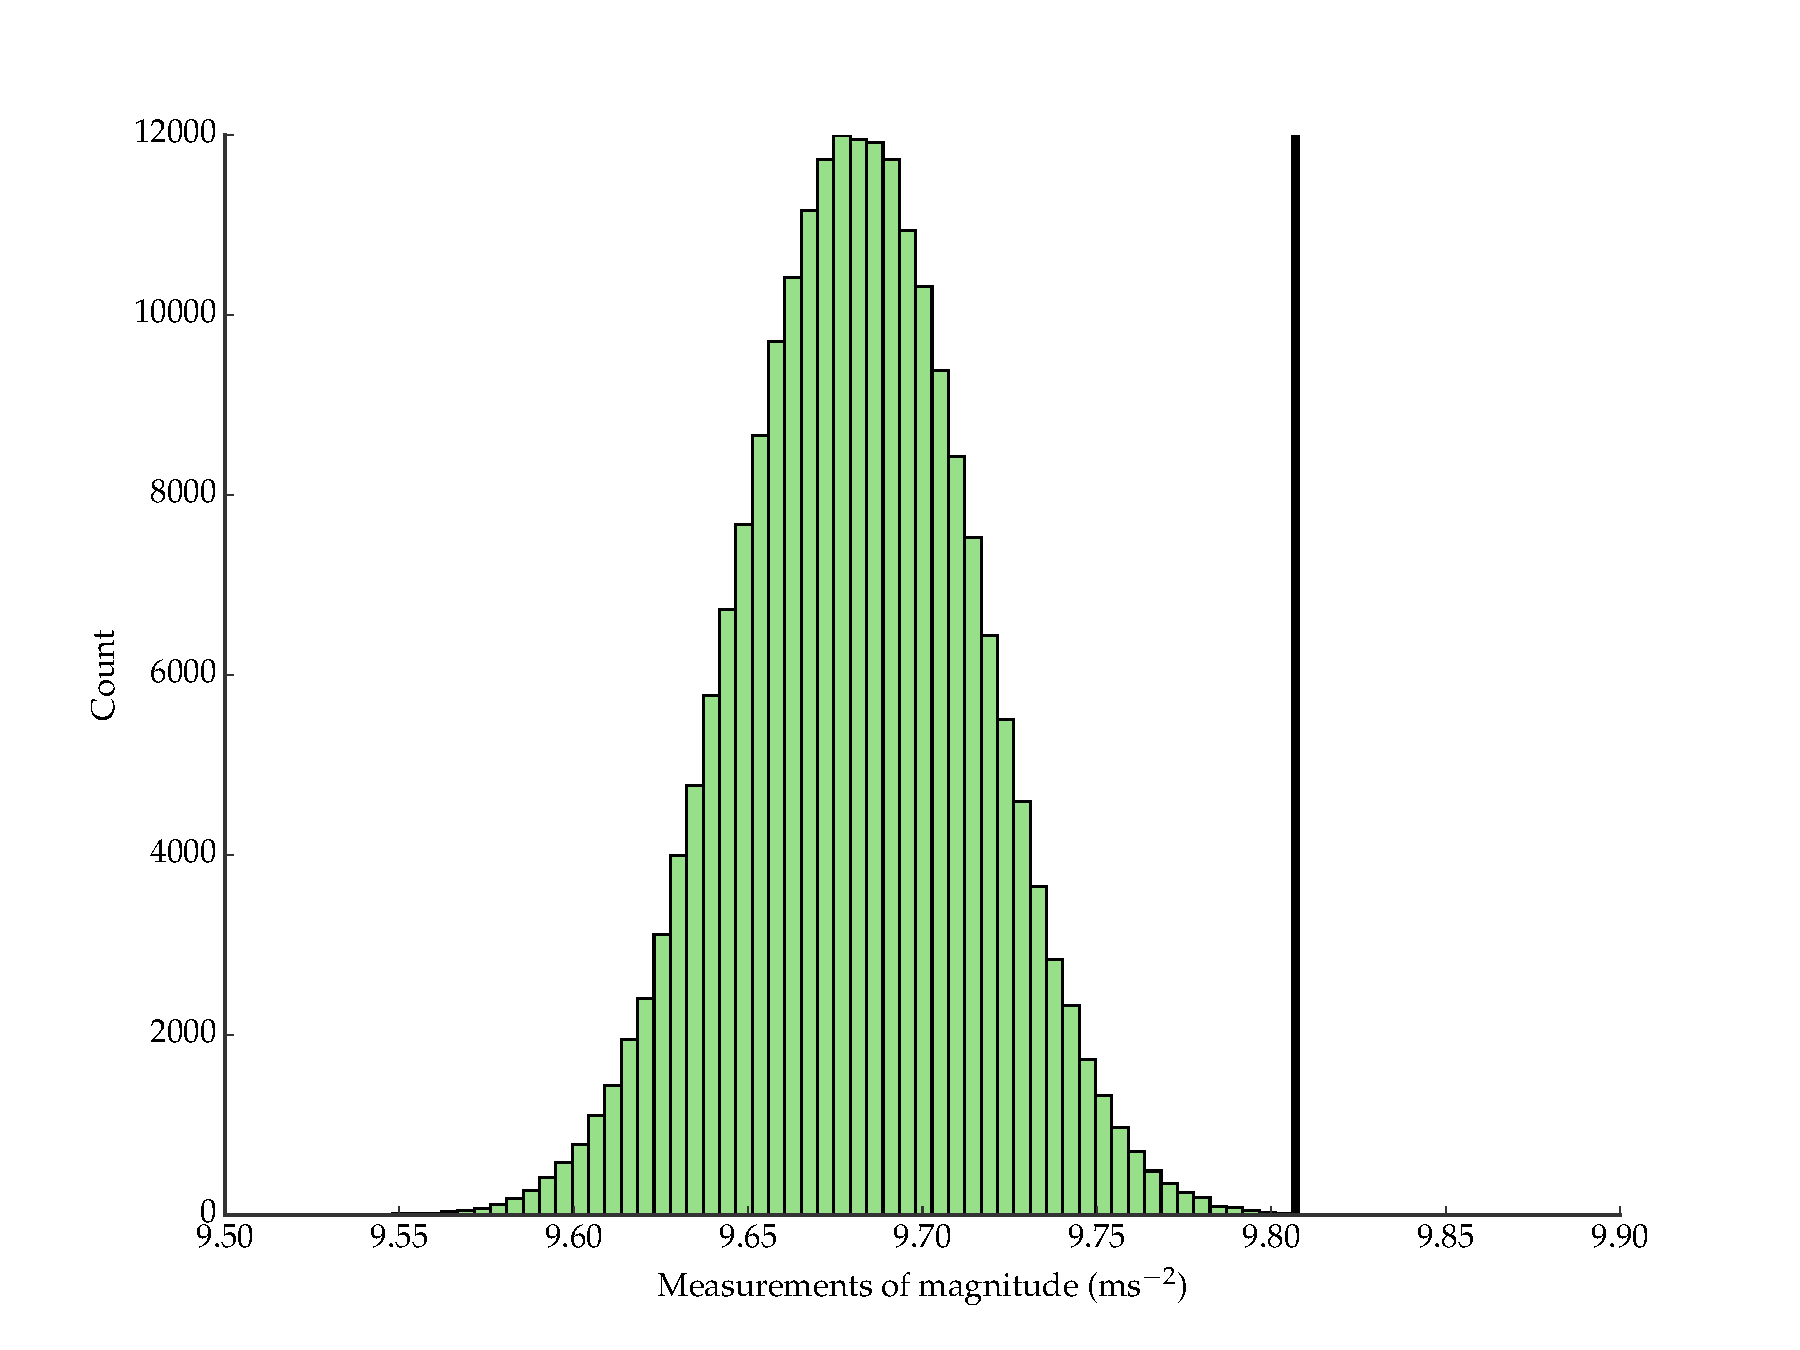
\includegraphics[width=0.8\textwidth]{noise_histogram}
        \caption{Histogram of the magnitude $\|\mathbf{x}\| = \sqrt{x^2+y^2+z^2}$ from the data shown in Figure~\ref{fig:x_y_z_flat_plot}. The magnitude should measure $ \mathrm{g} \approx 9.81\si{\metre\per\square\second}$. The noise implies the accelerometer data is imprecise. The mean of the data is less than $\mathrm{g}$, which indicates the recording is also inaccurate.}
        \label{fig:noise_histogram}
      \end{figure}
      
      Figure~\ref{fig:noise_prob_plot} gives a normal probability plot of the same magnitude data. Points on a normal probability plot should form a straight line if they are normally distributed. The straight line of best fit exhibits a coefficient of determination, $R^2$, which is very close to 1 and therefore it is very likely that the noise is normally distributed.
      
      \begin{figure}
        \centering
        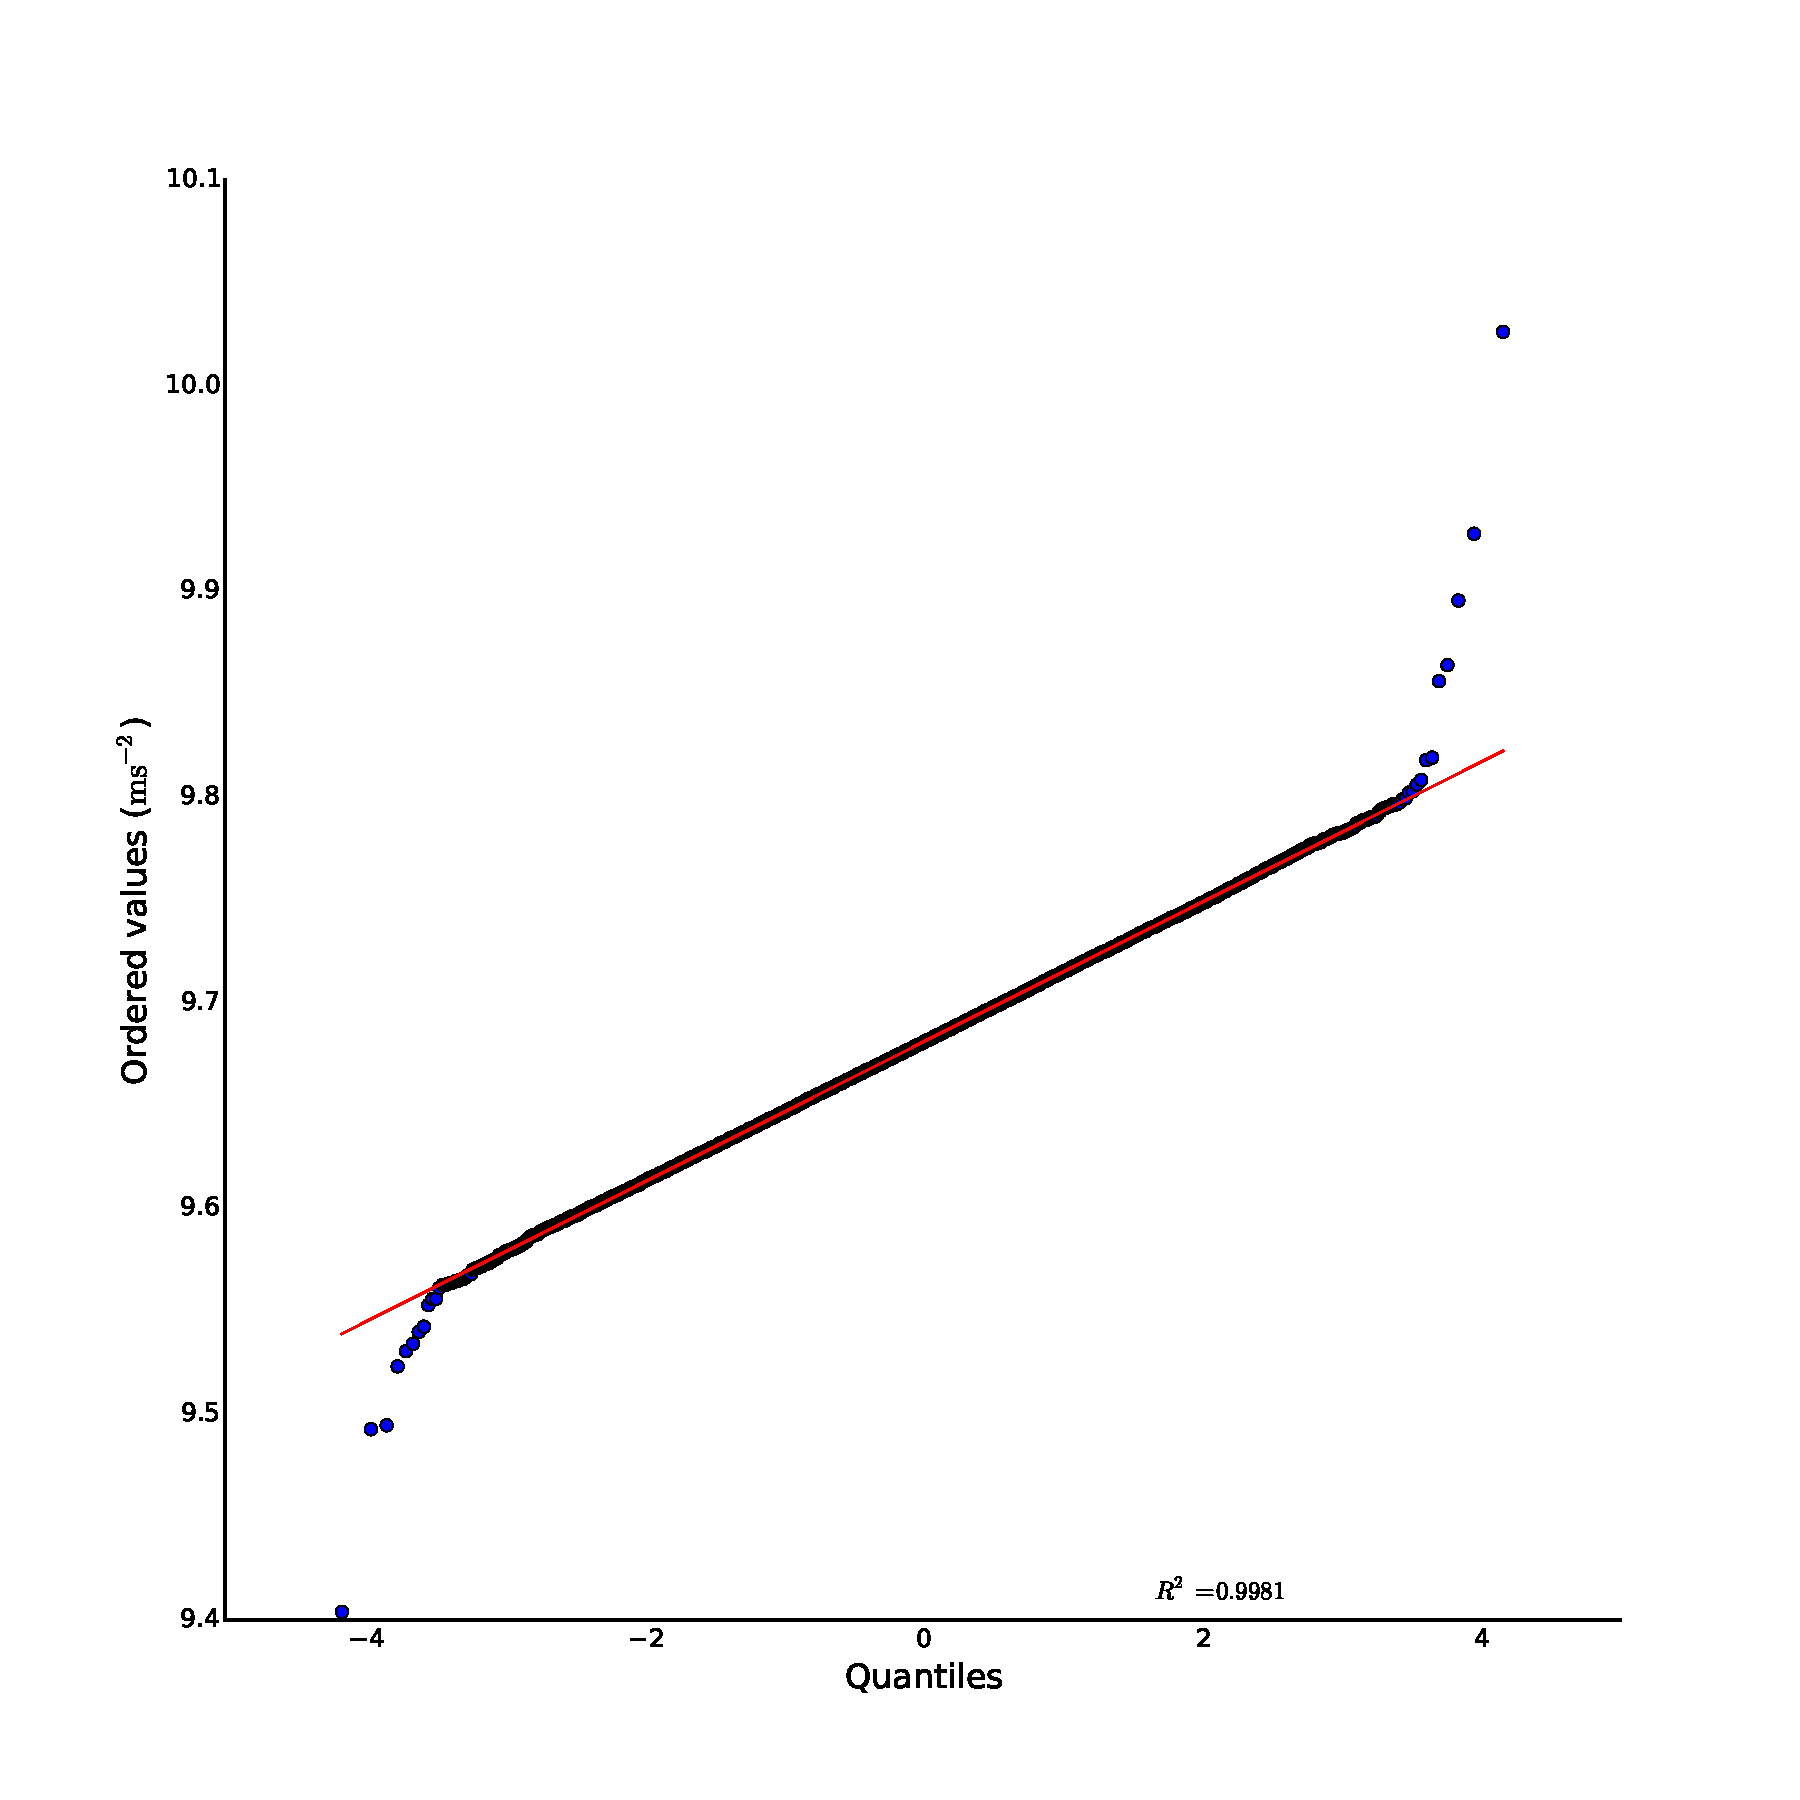
\includegraphics[width=0.8\textwidth]{noise_prob_plot}
        \caption{A normal probability plot of the magnitude $\|\mathbf{x}\| = \sqrt{x^2+y^2+z^2}$  from the data shown in Figure~\ref{fig:x_y_z_flat_plot}. Data that is normally distributed will form a straight line when plotted in this way. This data is very likely to be normally distributed, as indicated by the straight line.}
        \label{fig:noise_prob_plot}
      \end{figure}
      
      %TOOD: http://docs.scipy.org/doc/scipy/reference/generated/scipy.stats.probplot.html
      
      Noise can be reduced with the application of a low-pass filter. A low-pass filter attenuates signals with a higher frequency than some cutoff, such as the noise exhibited in the signal.
      
      %TODO: explain how filters work?
  
  \section{Hardware devices}
    The success of this project depends partly on correct selection and understanding of the devices
    used to collect data. Both the smartwatch and the smartphone are required to contain accelerometers accessible to
    developers.
    
    Android devices were chosen as Android Wear was the most mature platform for developing with
    wearable devices at the time. It runs on the widest variety of devices and provides developer 
    access to its sensors.
    
    \subsection{Smartphone}
      The smartphone chosen for development was the Google Nexus 5. Smartphone technology has
      advanced to the point that many Android smartphones are homogeneous with respect to this
      project --- they all contain sufficient processing power, internal memory and an 
      accerometer capable of recording data.
      
      The Nexus 5 contains a tri-axial accelerometer capable of recording measurements $\pm2\si{g}$
      on each axis, where $\si{g} \approx 9.81\si{\metre\per\square\second}$. This gives a total possible magnitude of $\sqrt{3 \times (2\mathrm{g})^2} = 2\mathrm{g}\sqrt{3} \approx 34 \si{\metre\per\square\second}$. Many other smartphones are susceptible to this limit and it is not thought that this will be an issue for classification.
      
      Figure~\ref{fig:nexus-5-accelerometer} shows the front face of a Nexus 5 with the axes of the
      accelerometer labeled.
      
      \begin{figure}[!th]
        \centering
        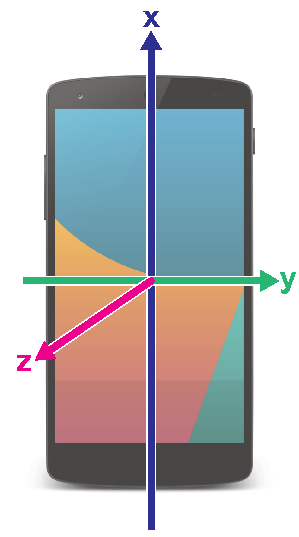
\includegraphics[width=0.3\textwidth]{Nexus_5_Accelerometer}
        \caption{A Nexus 5 device, overlayed with the coordinate system used by the Android API. The positive $x$ direction is defined as towards the top of the phone, the positive $y$ direction is defined as towards the right of the phone and the positive $z$ direction comes out of the screen. These directions are all relative to the natural portrait orientation of the device; they do not change when the device is used in horiztonal orientation.}
        \label{fig:nexus-5-accelerometer}
      \end{figure}
      
      %TODO: include tech specs of Nexus 5?
    
    \subsection{Smartwatch}
      \label{sec:smartwatch}
      The smartwatch chosen for development was the Samsung Galaxy Gear Live, running Android Wear.
      It pairs to any device running Android 4.4 or higher and communicates over Bluetooth.
      
      Wearable devices that do not run Android typically run either Tizen, an open-source but not 
      widely adopted operating system, such as the Samsung Galaxy Gear 2, or a proprietary 
      operating system that does not allow access to the raw accelerometer data, for example the 
      Jawbone Up.
      
      There is more differentiation in smartwatches than there is in smartphones, with them varying
      not just in screen size but also in screen format (round or rectangular), battery life,
      charging facilities and sensors. Table~\ref{tab:smartwatch-features} presents an overview of possible smartwatch devices.
      
      Though the Sony Smartwatch 3 has the best technical stats, it wasn't yet fully released at the time we acquired the smartwatch. The group has had previous success with Samsung devices and the Gear Live met all the requires I had of the smartwatch for the project.
      \begin{table}
        \centering
        {\tabulinesep=1.2mm
        \begin{tabu} to \linewidth { p{2cm} X[l] X[l] X[l] X[l]}
          Device & \textbf{Samsung Galaxy Gear Live} & \textbf{Samsung Galaxy Gear 2} &\textbf{ LG G Watch} & \textbf{Sony Smartwatch 3} \\
          \hline
          Operating System & Android Wear & Tizen & Android Wear & Android Wear \\
          \hline
          Processor & 1.2 GHz single-core Qualcomm Snapdragon 400 & 1.0 GHz dual-core Exynos 3250 & 1.2 GHz single-core Qualcomm Snapdragon 400 & 1.2 GHz quad-core ARM A7 \\
          \hline
          Memory & 512 MB RAM & 512 MB RAM & 512 MB RAM & 512 MB RAM \\
          \hline
          Storage & 4 GB & 4 GB & 4 GB & 4 GB \\
          \hline
          Sensors & Touchscreen, Accelerometer, Gyroscope, Compass, Heart Rate Monitor & Touchscreen, Accelerometer, Gyroscope, Heart Rate Sensor, 2 MP Camera & Touchscreen, Accelerometer, Gyroscope, Compass & Touchscreen, Accelerometer, Gyroscope, Compass \\
          \hline
          Radios & Bluetooth 4.0 Low Energy & Bluetooth 4.0 Low Energy & Bluetooth 4.0 Low Energy & Bluetooth 4.0 Low Energy, GPS, NFC, Wi-Fi \\
          \hline
          Battery & 300 mAh & 300 mAh & 400 mAh & 420 mAh \\
          \hline
          Notes &  & Pairs only with Samsung devices &  & \\
          \hline
          
        \end{tabu}}
        \caption{An overview of possible smartwatch devices. The Samsung Galaxy Gear Live was the device eventually chosen.}
        \label{tab:smartwatch-features}
      \end{table}
    
  \section{Libraries and APIs}
      This project makes use of existing libraries and APIs for the data collection, data handling
      and classification aspects of the project. I investigate each library and API early on to ensure I don't encounter any potential show-stopping issues further along. 
    
    \subsection{Android Sensor API}
      \label{sec:sensor-api}
      The Android platform Sensor API is implemented using a publisher-subscriber model. Listeners must be registered
      to a particular sensor and must implement an \texttt{onSensorChanged()}
      method. The \texttt{onSensorChanged()} method is called whenever the sensor reports a new 
      value. A \texttt{SensorEvent} object is provided, containing a timestamp at which the data was
      reported together with the new data.
      
      The rate at which \texttt{onSensorChanged()} is called is `user-suggested'; though it can be 
      specified by the user, it can also be altered by the Android system. In practice, this means
      that the difference in timestamps is not constant but is approximately equal to the specified 
      delay. A histogram of timestamp differences for a particular 1 hour recording is given in 
      figure~\ref{fig:timestamp-differences}.
      
      \begin{figure}[h]
        \centering
        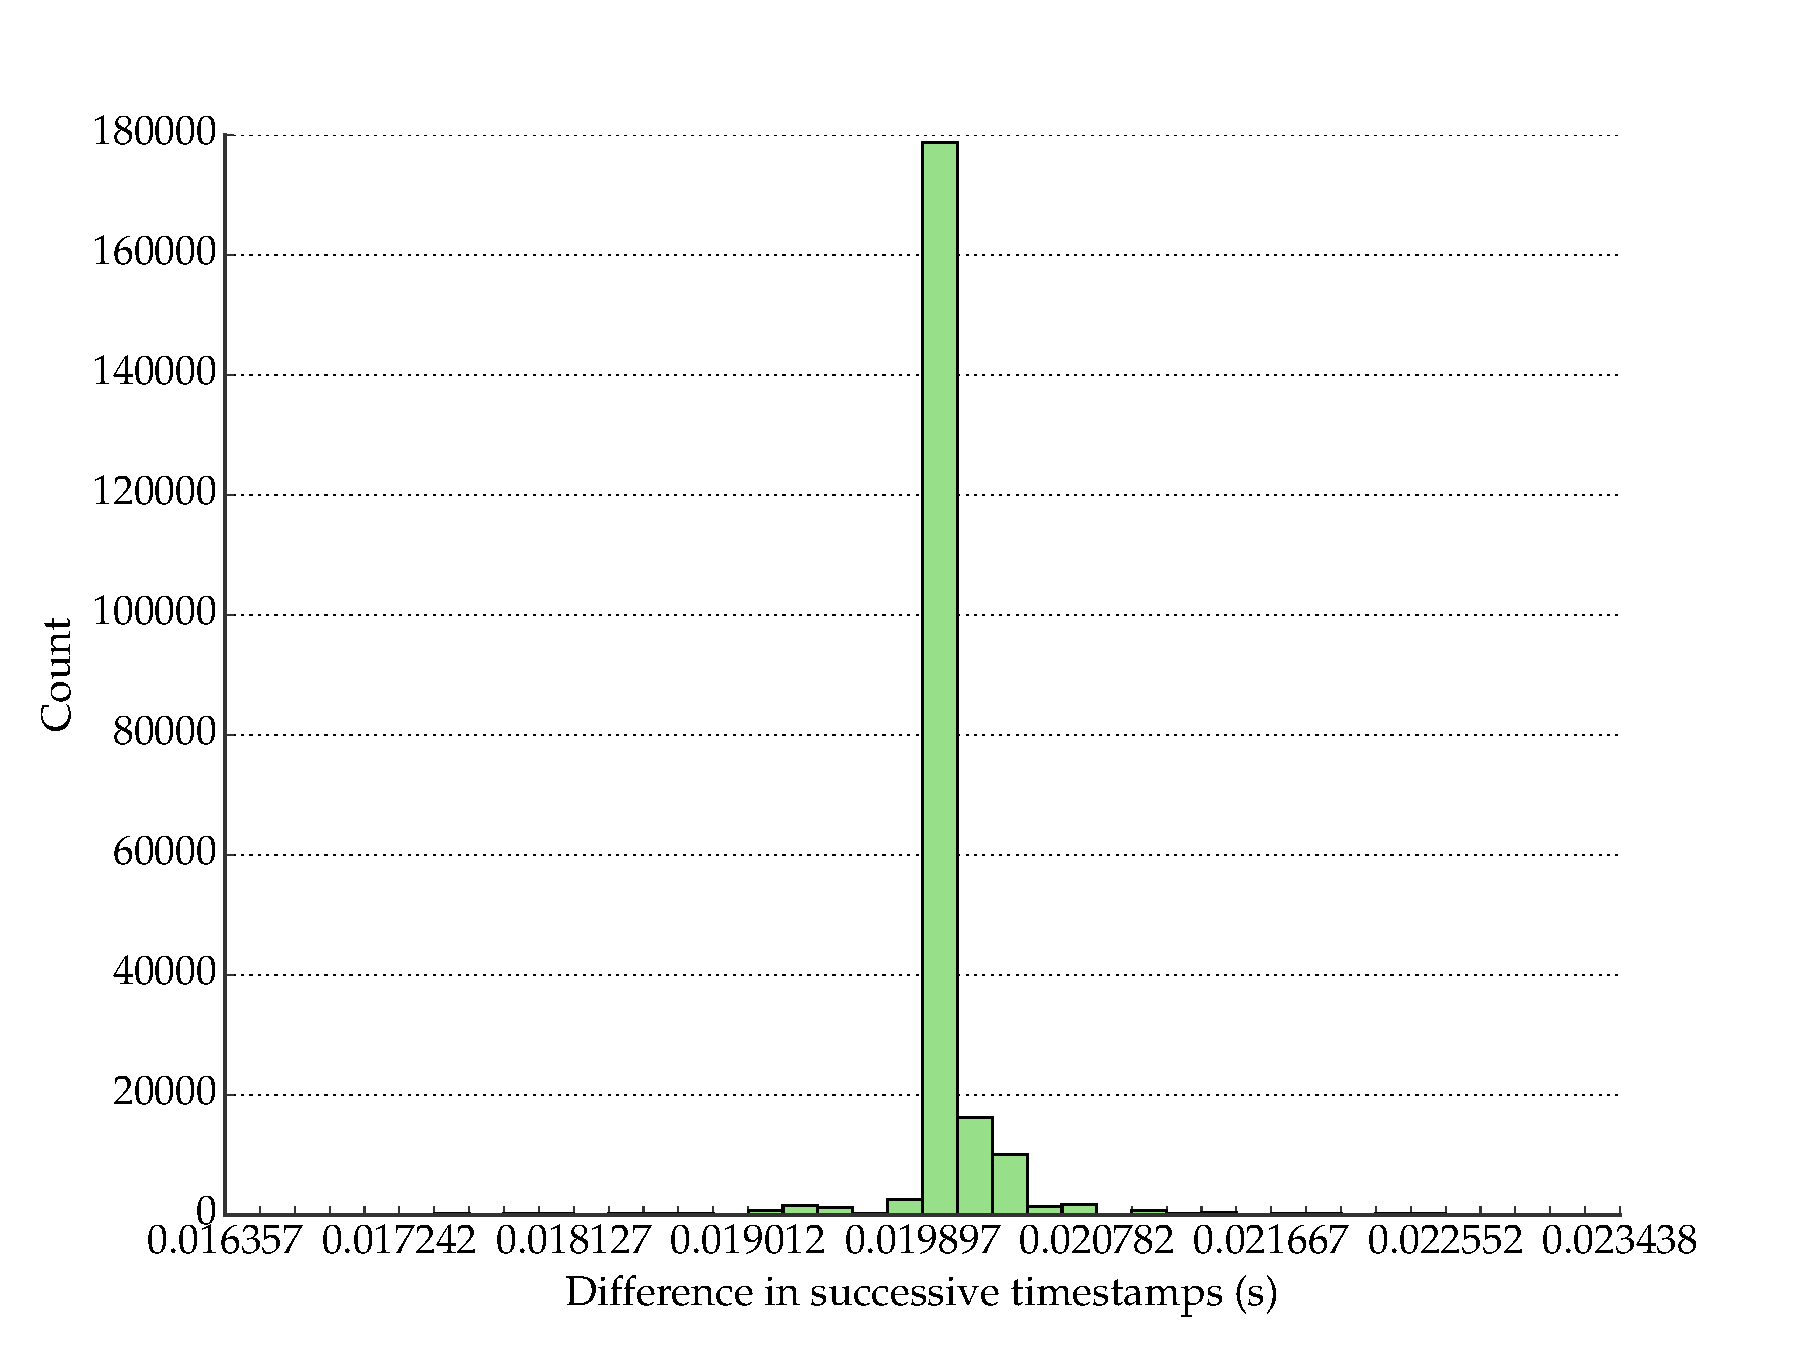
\includegraphics[width=0.8\textwidth]{timestamp_histogram}
        \caption{Histogram of the differences in successive timestamps of a one hour accelerometer 
            recording from the Nexus 5 smartphone. 
            The sample rate was set to 50 \si{Hz}. 0.02002s accounted for 75\% of the 
            differences.
            Thus the actual sample rate is approximately the user-suggested sample rate.}
        \label{fig:timestamp-differences}
      \end{figure}
      
      Android provides both acceleration and linear acceration sensors, related by 
      $$\textrm{acceleration} = \textrm{linear acceleration} + \textrm{gravity}$$
      They each provide a timestamp represented as a 64-bit integer (i.e. a long) and three 32-bit float values representing the 
      acceleration of each axis in \si{\metre\per\square\second} at that timestamp.   
      Table~\ref{tab:data-row} gives a graphical representation of the data returned.
      
      \begin{table}
        \centering
        \begin{tabu} to \linewidth {|X[2,c] | X[c] | X[c] | X[c] |}
          \hline
          Timestamp & X acceleration & Y acceleration & Z acceleration \\
          \si{ns} & \si{\metre\per\square\second} & \si{\metre\per\square\second} & \si{\metre\per\square\second} \\
          Long & Float & Float & Float \\
          2 bytes & 1 byte & 1 byte & 1 byte \\
          \hline
        \end{tabu}
        \caption{Data from the accelerometer sensor provided to the \texttt{onSensorChanged()} 
            method.}
        \label{tab:data-row}
      \end{table}
      
      Curiously, the timestamp returned as part of the data is documented only as ``The time in nanosecond [sic] at which the event happened'' \cite{androidsensoreventapi}. Futher exploration reveals that the timestamp is not defined against any particular zero-base, but rather the time since the device was powered on \cite{androidissuedocumentationbug, androidissuehardwarebug}. The implication of this for the project is that while the timestamp can be relied on for intervals between measurements, it cannot be used between different sets of recordings or across devices.
      
      %TODO: which are the x y z values of the device's accelerometer?
      
    \subsection{ES Sensor Manager}
      I explored this but didn't end up using it. Should I write about what it is and why I didn't
      end up using it?

    \subsection{Android Wear Data API}
      \label{sec:prep-data-api}
      As discussed in section~\ref{sec:smartwatch}, the only radio present in the Samsung Galaxy 
      Gear Live is Bluetooth. To transfer any recorded data from the watch, it must first be transferred to the paired smartphone. 
      The Android Wearable Data Layer API allows communication between Android handheld and wearable
      devices. It provides three methods of communication between devices:
      \begin{description}
        \item[Data items] provide data storage with automatic syncing;
        \item[Messages] are good for remote procedure calls but do not carry data;
        \item[Asset objects] for sending binary blobs of data.
      \end{description}
      
      %TODO: explain this as a diagram with state machine: recording state, recording off state
      The data layer synchronises data between the handheld and wearable. To do so, the Wearable Data Layer API requires the registration of a listener service, much like the Sensor API. The listener service listens for data layer events, such as the creation of asset objects or when messages are received.      
      
  \section{Choice of tools}
    \subsection{Programming languages}
      \label{sec:programming_languages}
      Java was chosen as it is the native programming language used on Android. Although it is
      possible to write code for Android in programming languages other than Java, for example 
      by using the Java Native Interface, doing so would not benefit the project. Java is taught in
      Part 1A and Part 1B of the Computer Science Tripos. The Android SDK builds on principles
      covered in the course but is complicated by having to manage interactions with the Android operating system.
      
      XML is Android's standard markup language. All user-interface components are written in XML.
      The project includes a user interface to configure and control the recording of data.
      
      Python 3.4 was chosen as the data processing language due to its ease of use and the strength of its data processing, signal processing and machine learning libraries:
      \begin{description}
        \item[NumPy:] a scientific computing library and the basis for the other three libraries below.
        \item[Pandas:] extensions to NumPy that enable easier processing of time-series data.
        \item[SciPy:] signal processing tools and other statistical features.
        \item[Scikit Learn:] machine learning classifiers and utilities to work with them.
      \end{description}
      All of NumPy, SciPy, Pandas and Scikit Learn are open-source and licensed under the BSD license.
    \subsection{Development Environment}
      Two powerful IDEs, Android Studio and PyCharm were used for the development of the Android app and the Python data pipeline respectively. Android Studio is available for free from Google, while PyCharm is provided free for educational use by JetBrains. Both include advanced debuggers.
      
      Though the Android SDK contains a device emulator, it runs slowly and cannot simulate sensors. Developing the Android apps is therefore done by connecting them to a computer and running new versions of the code. This also enables access to the device's logs from the development environment. I made extensive use of logging to determine that the program was executing as expected.
  \section{Software engineering techniques}
    \subsection{Development methodologies}
      I used a combination of development methodologies for the project. The data collection apps were developed using a waterfall methodology, while the data processing was developed using an Agile methodology.
      
      Waterfall models are excellent when the end goals of the project are known and can be well specified. The goal of the data collection apps can be easily stated: to write apps for the smartphone and smartwatch that will allow user collection of accelerometer data.
      
      The data processing and machine learning elements of the project required an Agile methodology. The goal here is less well defined --- to classify activities with the greatest accuracy --- and the implementation to achieve the goal is far more experimental.
      
    \subsection{Version control and backups}
      I used three separate Git repositories for the data collection code, the data processing code and the dissertation respectively. The Git repositiories were synced to GitHub at each commit. Version control allowed me to follow a \emph{implement--test--commit} pattern when writing code. 
      
      GitHub also served as one method of backup. Each GitHub repository is publicly accessible such that I can continue implementation even if my primary development computer crashed and I was also locked out of my GitHub account. In addition, I backed up periodically to Dropbox and to an external hard drive. The external hard drive backup retained old copies of files when they were updated. This gives four replications of my entire project, with two of these able to access previous versions of the code.  
  \section{Summary}
    In this section I presented:
    \begin{itemize}
      \item an overview of digital signal processing;
      \item information on the smartphone and smartwatch used;
      \item details of key APIs used including the Android Sensor API and the Android Wear Data API;
      \item development tools and software engineering techniques.
    \end{itemize}
